


\section{Introduction}
\label{sec:I}
% 学习此类映射的可能性,为设计具有广泛适用性的深度学习框架开辟了一类新问题。传统神经网络是有限维欧氏空间(finite-dimensional Euclidean spaces)和 / 或有限基数集合(sets of finite cardinality)之间的映射,基于传统神经网络进行拓展需要新的思路。这涉及无穷维空间(infinite-dimensional spaces),例如输入和输出本身是定义在欧氏空间某一区域上的函数的情况。
学习函数空间(function spaces)之间的映射在科学与工程领域具有广泛应用。例如,在求解微分方程(differential equations)时,输入为系数函数(coefficient function),输出为解函数(solution function)。解决该问题的一种直接方法是将无穷维的输入和输出函数空间离散化(discretize)为有限维网格(finite-dimensional grids),并应用神经网络(neural networks)等标准学习模型。然而,这种方法会限制适用性,因为所学习的神经网络模型可能无法很好地泛化到训练数据离散化网格(discretization grid)之外的其他离散化(discretizations)情况。
为克服标准神经网络的这些局限性,我们构建(formulate)了一个用于学习算子的新型深度学习框架,称为 {\em 神经算子(neural operators)},它可直接在有界区域(bounded domains)上的函数空间之间进行映射。由于我们的神经算子是在函数空间上设计的,因此可以通过多种不同方法、在不同分辨率(resolution)水平下对其进行离散化,且无需重新训练。相比之下,标准神经网络架构严重依赖训练数据的离散化:对于不同离散化程度的数据,可能需要具有新参数的新架构才能达到相同的误差水平。我们还提出了 {\em 离散化不变(discretization-invariant)} 模型的概念(notion),并证明我们的神经算子满足该性质(property),而标准神经网络则不满足。
% 此类神经算子模型一旦训练完成,便具有离散化不变性质:可在基础函数数据的不同离散化形式之间共享相同的模型参数。我们通过数值实验证明,对于数据的任意离散化形式,同一神经算子都能实现低误差,而标准前馈神经网络(feed-forward neural networks)和卷积神经网络(convolutional neural networks)则无法做到。在偏微分方程(partial differential equations, PDEs)场景下,我们通过数值实验证明,在固定分辨率下,所提出的方法与神经网络模型相比具有很强的竞争力,且比用于生成数据的偏微分方程求解器(PDE solvers)快几个数量级(orders of magnitude)。
% 最后,我们为所提出的神经算子建立了通用逼近定理(universal approximation theorem),证明它们能够以任意精度逼近线性和非线性算子(linear and non-linear operators)。
% 本文研究了偏微分方程模型衍生的各类解算子(solution operators)或流映射(flow maps);具体而言,我们研究了函数空间之间的映射,其中输入数据例如可以是初始条件(initial condition)、边界条件(boundary condition)或系数函数,而输出数据则是相应的解。我们针对以下算子开展了数值实验:一维泊松方程(one-dimensional Poisson equation)\citep {Evans}、一维时间相关伯格斯方程(time-dependent one-space-dimensional Burgers' Equation)\citep {Evans}、二维稳态达西流动(two-dimensional steady Darcy Flow)\citep {bear2012fundamentals} 以及二维时间相关不可压缩纳维 - 斯托克斯方程(time-dependent two-space dimensional incompressible Navier-Stokes Equation)\citep {constantin1988navier,lemarie2018navier,temam2001navier}。
%3.1 节(Subsection \ref {ssec:LR})介绍了本文工作的研究背景与相关背景信息。3.2 节(Subsection \ref {ssec:OC})详细阐述了我们的研究贡献,并概述了论文内容。本文引言部分在 3.3 节(Subsection \ref {ssec:related-work})结束,该节提供了文献综述(literature review)。

%The possibility of learning such mappings opens up a new class of problems in the design of deep learning frameworks with widespread applicability. New ideas are required to build upon traditional neural networks which are mappings between finite-dimensional Euclidean spaces and/or sets of finite cardinality.   This involves infinite-dimensional spaces, such as the case where inputs and outputs are themselves functions over a domain in the Euclidean space

Learning mappings between  function spaces has widespread applications  in science and engineering. For instance, for  solving differential equations,  the input is a coefficient function and the output is a solution function. A straightforward solution to this problem  is to simply  discretize the infinite-dimensional input and output function spaces into finite-dimensional grids, and apply standard learning models such as 
neural networks. However, this limits  applicability since the learned  neural network model may not  generalize well to different discretizations, beyond the discretization grid of the training data.

To overcome these limitations of standard neural networks, we  formulate a new deep-learning framework for learning operators, called {\em neural operators}, which directly map between  function spaces on bounded domains.  Since our neural operator is  designed on function spaces, they
can be discretized by a variety of different methods, and at different levels of resolution, without the need for re-training. In contrast, standard neural network architectures depend heavily on the discretization of training data: new architectures with new parameters may be needed to achieve the same error for   data with varying discretization.  We also propose the notion of {\em discretization-invariant} models and prove that our neural operators satisfy this property, while standard neural networks do not. 

%Such neural operator models, once trained, have the  property of being  discretization invariant: it is possible to share the same model parameters among different discretization of the underlying functional data. We demonstrate, numerically, that the same neural operator can achieve a low error for any discretization of the data while standard feed-forward and convolutional neural networks cannot. In the context of partial differential equations (PDEs) we demonstrate numerically that, at fixed resolution, the resulting methods are highly competitive when compared with neural network models and are orders of magnitude faster than the PDE solvers used to generate data. 

%Finally we establish a universal approximation theorem for the neural operators we introduce, proving their ability to approximate linear and non-linear operators arbitrary well.

%In this paper we study various solution operators or flow maps arising from PDE models; in particular, we investigate  mappings between function spaces where the input data can be, for example, the initial condition, boundary condition, or coefficient function, and the output data are the respective solutions. We perform numerical experiments with operators arising from the one-dimensional Poisson equation \citep{Evans}, the time-dependent one-space-dimensional Burgers' Equation \citep{Evans},  two-dimensional steady Darcy Flow \citep{bear2012fundamentals} and the time-dependent two-space dimensional incompressible Navier-Stokes Equation \citep{constantin1988navier,lemarie2018navier,temam2001navier}.

%Subsection \ref{ssec:LR} contains background and context for our work. Subsection \ref{ssec:OC} details our contributions and outlines the contents of the paper. We conclude this introduction in Subsection \ref{ssec:related-work} which provides a literature review. 


\subsection{Our Approach}
\label{ssec:OC}



\paragraph{Discretization-Invariant Models.}

We formulate a precise mathematical notion of discretization invariance. We require any discretization-invariant model with a fixed number of parameters to satisfy the following:
\begin{enumerate}[leftmargin=*]
    \item  acts on any discretization of the input function, i.e. accepts any set of points in the input domain,
    \item can be evaluated at any point of the output domain,
    \item  converges to a continuum operator as the discretization is refined. 
\end{enumerate} 



\noindent The first two requirements of accepting any input and output points in the domain is a natural requirement for discretization invariance, while the last one ensures consistency in the limit as the discretization is refined. For example, families of graph neural networks~\citep{scarselli2008graph} and transformer models~\citep{vaswani2017attention} are resolution invariant, i.e., they can receive inputs at any resolution, but they fail to converge to a continuum operator as discretization is refined. Moreover, we require the models to have a fixed number of parameters; otherwise, the number of parameters becomes unbounded in the limit as the discretization is refined, as shown in Figure \ref{fig:discretization-invariance}.  Thus the notion of discretization invariance allows us to define neural operator models that are consistent in function spaces and can be applied to data given at any resolution and on any mesh. We also establish that standard neural network models are not discretization invariant.

% \todo{zongyi: can u add fig for mesh refinement for air foil. it is fine that it is irregular. we are defining notion here. }

%\begin{figure}[h]
%\includegraphics[width=\textwidth]{}
%\end{figure}



\begin{figure}[h]
    \centering
    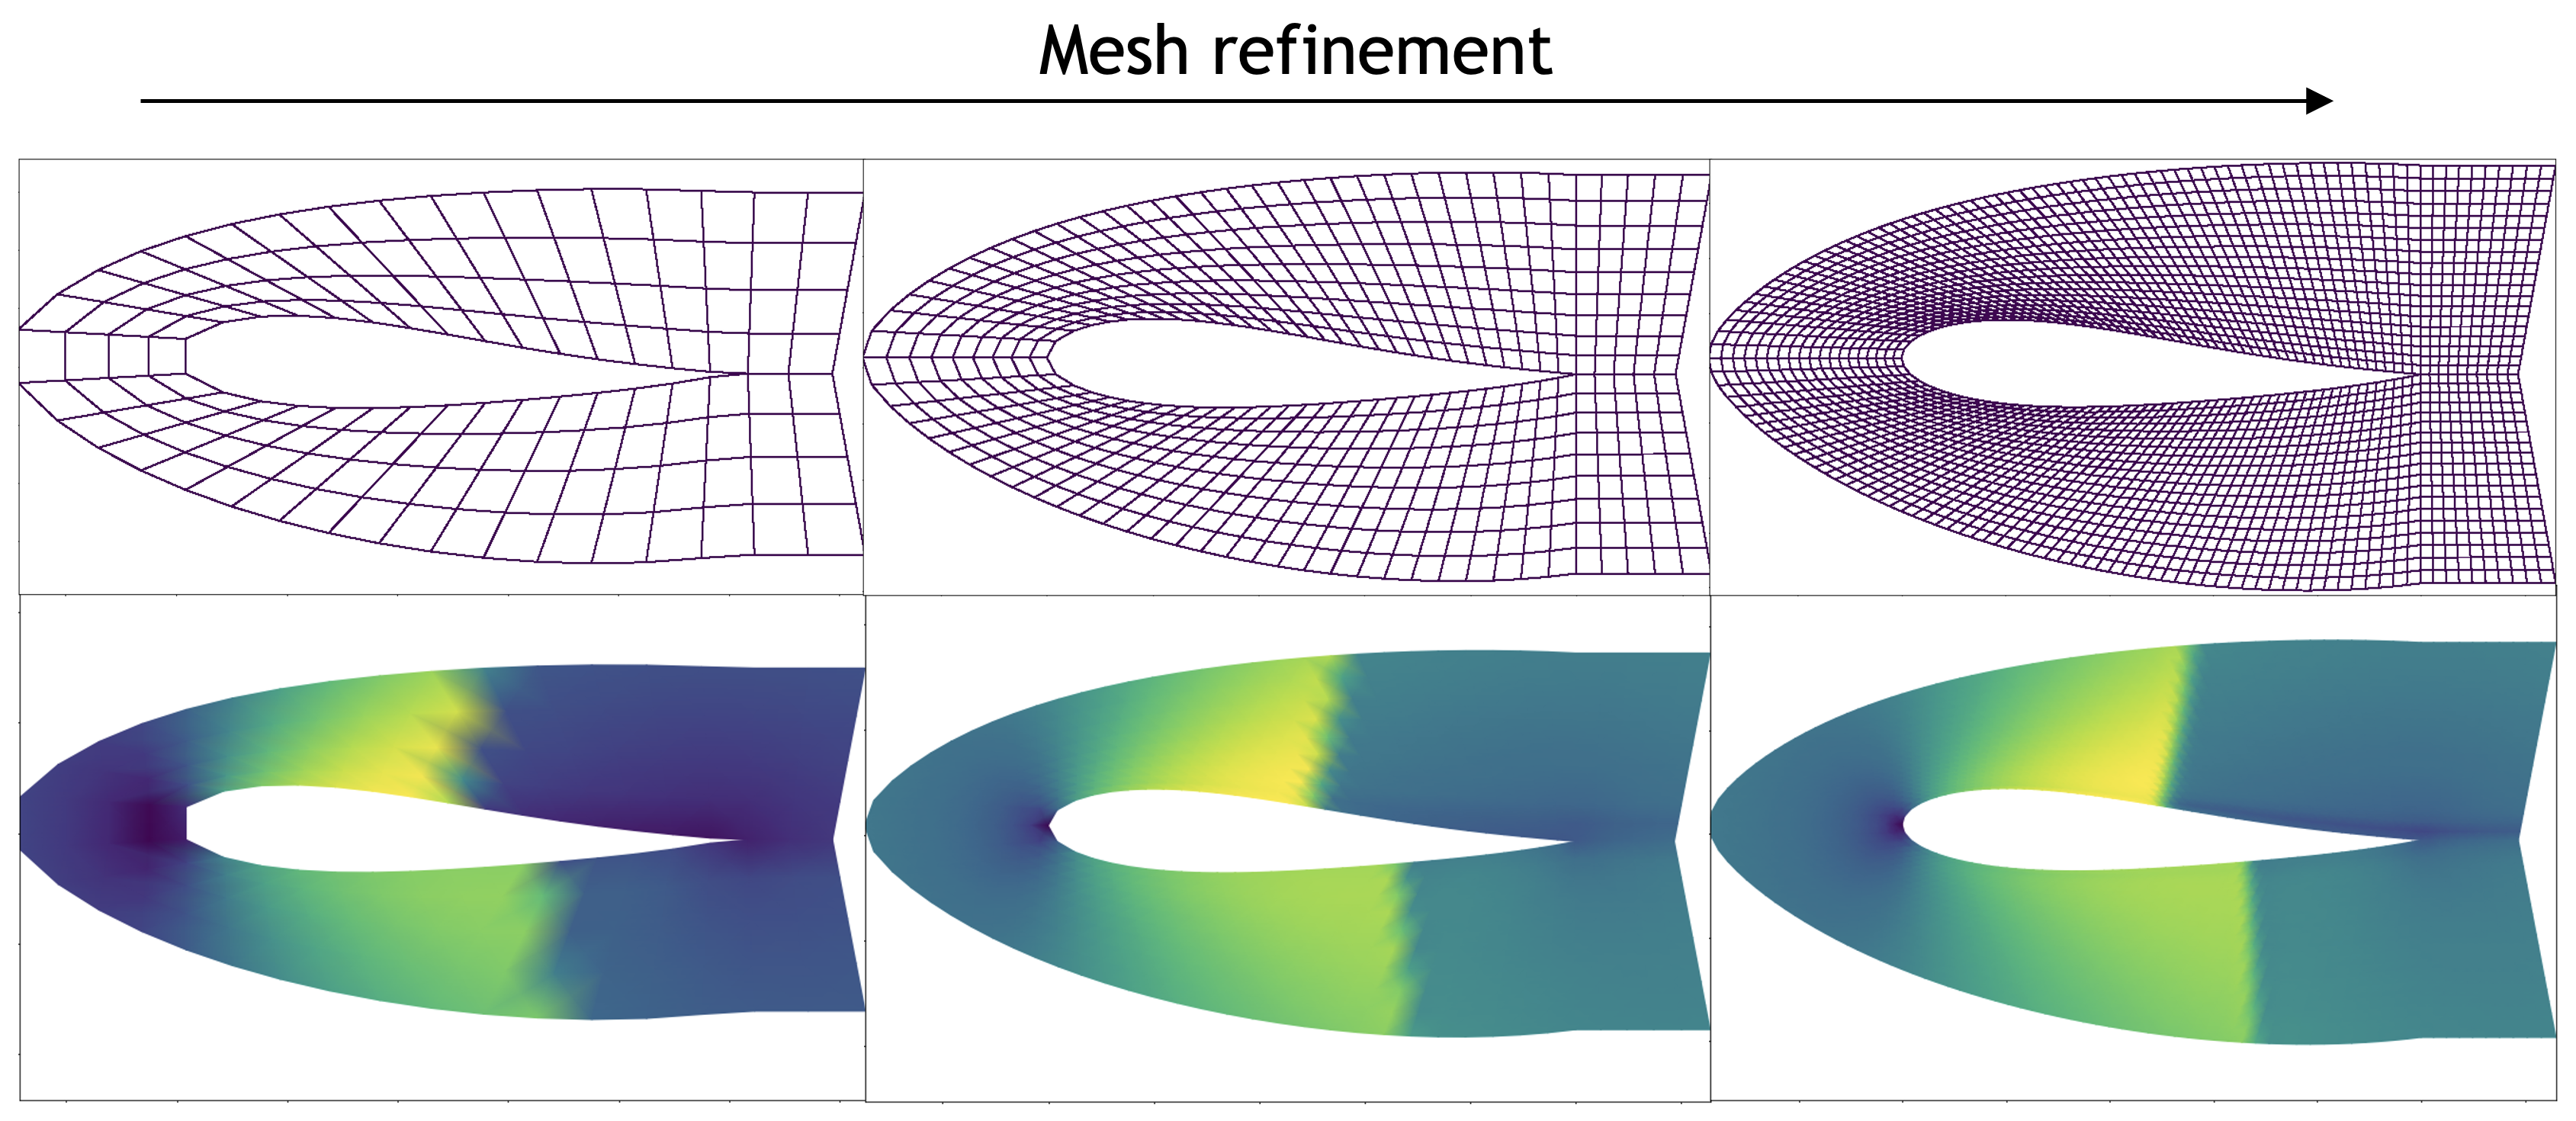
\includegraphics[width=0.8\textwidth]{Figs/discretization-invariance.png}
    \caption{Discretization Invariance}
    \label{fig:discretization-invariance}
    An discretization-invariant operator has convergent predictions on a mesh refinement.
\end{figure}

\paragraph{Neural Operators.}


We introduce the concept of neural operators   for learning operators that are  mappings between infinite-dimensional function spaces. We propose neural operator architectures to be multi-layers where layers  are themselves operators composed with non-linear activations. This ensures that that the overall end-to-end composition  is an operator, and thus satisfies the discretization invariance property. The key design choice for neural operator is the operator layers. To keep it simple, we limit ourselves to layers that are linear operators. Since these layers are composed with non-linear activations, we obtain neural operator models that are expressive and able to capture any continuous operator. The latter property is known as universal approximation. 

The above line of reasoning for neural operator design follows closely the design of standard neural networks, where linear layers (e.g. matrix multiplication, convolution) are composed with non-linear activations, and we have universal approximation of continuous functions defined on compact domains~\citep{hornik1989multilayer}. Neural operators replace finite-dimensional linear layers in neural networks with linear operators in function spaces.


%We further show that neural operators models are universal approximators of operators acting between Banach spaces. It is well known that neural networks are universal approximators of functions, meaning that they can uniformly approximate any continuous function defined on a compact domain~\citep{hornik1989multilayer}. We analogously show that neural operators can uniformly approximate any continuous operator defined on a compact set of a Banach space. 
%Due to the generality of neural operators, it is desirable to study whether neural operators can approximate any operator. 

%\begin{theorem}[Universal approximation of operators]
%\label{thm:univ_approx_informal}
%Neural operators are universal approximators of operators. Given proper input and output function spaces, neural operators approximate any operator arbitrary accurately on an appropriate topology.
%\end{theorem}
%The formal statements of this, and related theorems, are provided in Subsection~\ref{sec:approximation_main}; proofs are in an appendix. %This theorem express that when using neural operators to approximate an operator in practice, one may not be concerned with the capacity of the model class from the approximation theoretic point of view. 



%\paragraph{Properties of Neural Operators.}


%\begin{theorem}[Discretization invariance of neural operators]
%\label{thm:disc_inv_informal}
%Neural operators satisfy the above criteria of being discretization-invariant and a fixed neural operator model can act on any discretization used to represent the input function. 
%\end{theorem}
%The formal statement of this theorem is provided in Subsection~\ref{sec:discritizational_invariance} with related discussion in Section~\ref{sec:neuraloperators}. 
%In this paper, we show that traditional neural networks are not discretization invariant models, while slightly modified transformers are resolution invariant models. 




We  formally establish that neural operator models with a fixed number of parameters satisfy discretization invariance. We further show that neural operators models are universal approximators of continuous operators acting between Banach spaces, and  can uniformly approximate any continuous operator defined on a compact set of a Banach space.   {\bf Neural operators are the only known class of models that guarantee both discretization-invariance and universal approximation.} See Table~\ref{table:deeplearning_comparison} for a comparison among the deep learning models. Previous deep learning models are mostly defined on a fixed grid, and  removing, adding, or moving grid points generally makes these models no longer applicable. Thus, they are  not discretization invariant. 


We propose several design choices for the linear operator layers in neural operator such as a parameterized integral operator or through multiplication in the spectral domain as shown in Figure~\ref{fig:NO_architecture}.  
Specifically, we propose four practical methods for implementing the neural operator framework: graph-based operators, low-rank operators, multipole graph-based operators, and Fourier  operators. Specifically, for graph-based operators, we develop a Nystr\"om extension to connect the integral operator formulation of the neural operator to families of graph neural networks (GNNs) on arbitrary grids. For Fourier operators,  we consider the spectral domain formulation of the neural operator which leads to efficient algorithms in settings where fast transform methods are applicable. 

We include an exhaustive numerical study of the four formulations of neural operators. Numerically, we show that the proposed methodology consistently outperforms all existing deep learning methods even on the resolutions for which the standard neural networks were designed. For the two-dimensional Navier-Stokes equation, when learning the entire flow map,  the method achieves $<1\%$ error for a Reynolds number of 20 and $8\%$ error for a Reynolds number of 200.

The proposed Fourier neural operator (FNO) has an inference time that is three orders of magnitude faster than the pseudo-spectral method used to generate the data for the Navier-Stokes problem \citep{chandler2013invariant} -- $0.005$s compared to the $2.2s$ on a $256 \times 256$ uniform spatial grid. %\todo{need to change this}
Despite its tremendous speed advantage, the method does not suffer from accuracy degradation when used in downstream applications such as solving Bayesian inverse problems. Furthermore, we demonstrate
that FNO is robust to noise on the testing problems we consider here.

\begin{figure}[t]
    \centering
    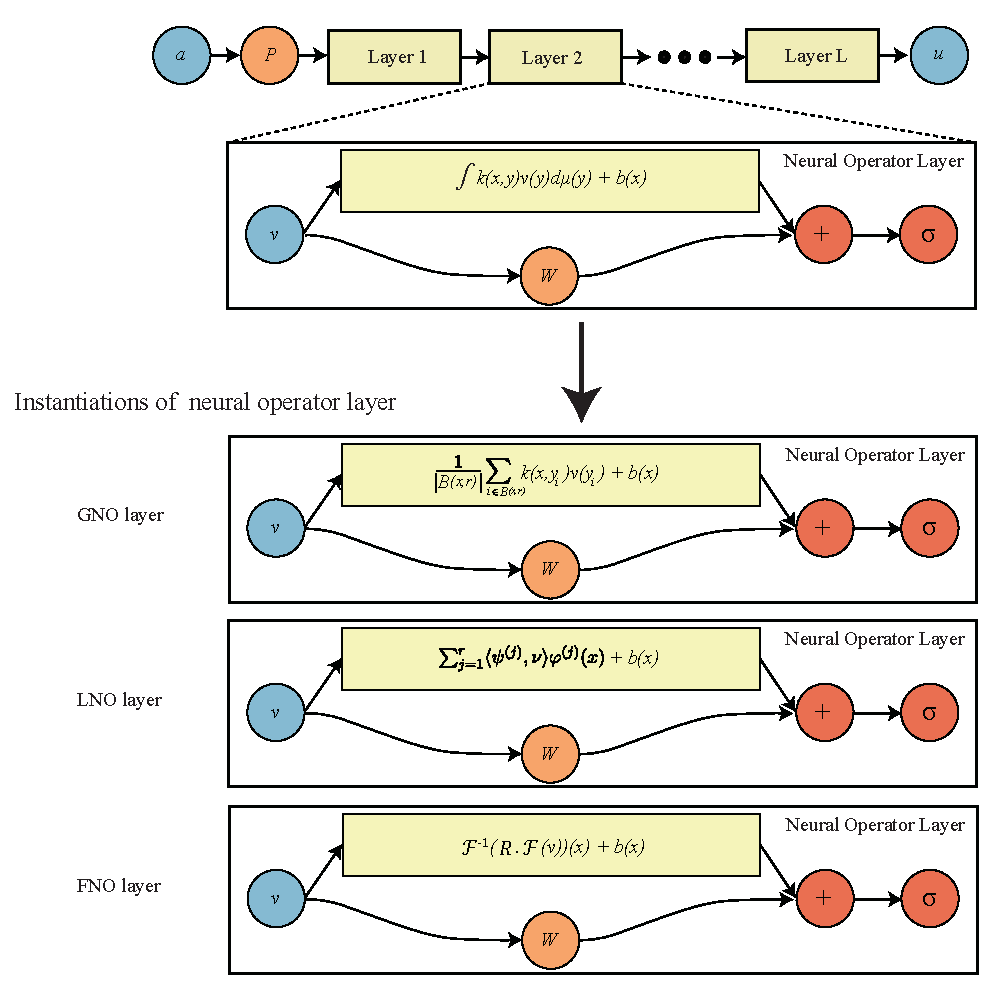
\includegraphics[width=0.8\textwidth]{Figs/NO-all-eq.pdf}
    \caption{Neural operator architecture schematic}
    \label{fig:NO_architecture} 
    \small{The input function $a$ is passed to a pointwise lifting operator $P$ that is followed by $T$ layers of integral operators and pointwise non-linearity operations $\sigma$. In the end, the pointwise projection operator $Q$ outputs the function $u$. Three instantiation of neural operator layers, GNO, LNO, and FNO are provided.}
\end{figure}



%This is undesirable since, in many scientific and engineering applications, function evaluations are often sensory and provided on varying per-sample grid points. In contrast, the discretization property of neural operators allows them to be defined and operator on varying grid locations and sizes, desirable characteristics for the downstream tasks. 


% \begin{table}[h!]
% \centering
% \begin{tabular}{l|c|c|c|c}
% % \diaghead{Scoreexp}{Property}{Model}&
% \diagbox{Property\hspace{.5cm}}{\hspace{2em}\raisebox{-.3cm}{Model}}&
% CNNs& DeepONets & Interpolation & Neural Operators\\
% \hline
% Discretization Invariance & \xmark & \xmark & \cmark & \cmark \\
% \hline
% Can the output function be queried at any point? & \xmark & \cmark & \cmark & \cmark \\
% \hline
% Input at any point & \nk{\cmark} & \xmark & \cmark & \cmark \\
% \hline
% Universal Approximation & \xmark & \cmark & \xmark & \cmark \\
% \hline
% \end{tabular}
% \caption{Comparison of deep learning models. The first row indicates whether the model is discretization invariant. The second and third rows indicate whether the output and input are a functions. The fourth row indicates whether the model class is a universal approximator of operators. Neural Operators are discretization invariant deep learning methods that output functions and can approximate any operator.}
% \label{table:deeplearning_comparison}
% \end{table}
% }


\begin{table}[h!]
\centering
\begin{tabular}{l|c|c|c|c}
% \diaghead{Scoreexp}{Property}{Model}&
\diagbox{Property\hspace{.5cm}}{\hspace{2em}\raisebox{-.3cm}{Model}}&
NNs& DeepONets & Interpolation & Neural Operators\\
\hline
Discretization Invariance & \xmark & \xmark & \cmark & \cmark \\
\hline
Is the output a function? & \xmark & \cmark & \cmark & \cmark \\
\hline
Can query the output at any point? & \xmark & \cmark & \cmark & \cmark \\
\hline
Can take the input at any point? & \nk{\xmark} & \xmark & \cmark & \cmark \\
\hline
Universal Approximation & \xmark & \cmark & \xmark & \cmark \\
\hline
\end{tabular}
\caption{Comparison of deep learning models. The first row indicates whether the model is discretization invariant. The second and third rows indicate whether the output and input are a functions. The fourth row indicates whether the model class is a universal approximator of operators. Neural Operators are discretization invariant deep learning methods that output functions and can approximate any operator.}
\label{table:deeplearning_comparison}
\end{table}



\subsection{Background and Context}
\label{ssec:LR}


\paragraph{Data-driven approaches for solving PDEs.}
%``Differential equations [...] represent the most powerful tool humanity has ever created for making sense of the material world.'' \citet{strogatz2009loves}. 
% A wide range of important engineering and physics problems are governed by PDEs. 
Over the past decades, significant progress has been made in formulating \citep{gurtin1982introduction} and solving \citep{johnson2012numerical} the governing PDEs in many scientific fields from micro-scale problems (e.g., quantum and molecular dynamics) to macro-scale applications (e.g., civil and marine engineering). Despite the success in the application of PDEs to solve real-world problems,  two significant challenges remain: (1) identifying the governing model for complex systems; (2) efficiently solving large-scale nonlinear systems of equations.

Identifying and formulating the underlying PDEs appropriate for modeling a specific problem usually requires extensive prior knowledge in the corresponding field which is then combined with universal conservation laws to design a predictive model. For example, modeling the deformation and failure of solid structures requires detailed knowledge of the relationship between stress and strain in the constituent material. For complicated systems such as living cells, acquiring such knowledge is often elusive and formulating the governing PDE for these systems remains prohibitive, or the models
proposed are too simplistic to be informative. The possibility of acquiring such knowledge from data can revolutionize these fields. 
Second, solving complicated nonlinear PDE systems (such as those arising in turbulence and plasticity) is computationally demanding and can often make realistic simulations intractable. Again the possibility of using instances of data to design fast approximate solvers holds great potential for accelerating numerous problems.

\iffalse
\subsection{Learning the Operator} We want to stress that learning the operator $\F$ is a more challenging task compared to finding the solution $u$ for a single equation. Most of the existing methods, ranging from traditional finite element methods (FEM), finite difference methods (FDM), to machine learning based physics-informed neural networks (PINNs) \citep{raissi2019physics}, they all aim to find $u$ for a single equation (i.e., single solving for a single $a$). On the other hand, we want to parameterize $\F$ as a mapping from $a\in\A$ to $u\in\U$.

Compared to PDE solvers such as FEM and PINNs, the neural operator learns the solution operator doesn't require to solve each equation separately. It immediately outputs the evaluation for any new query $a$. Therefore, it is usually used as a fast evaluator. For example, for inverse problem when one need to find some optimal material structures $a$, the neural operator can quickly evaluate input $a'$, combining with optimization methods to find $a' \to a$.
\fi 

\paragraph{Learning PDE Solution Operators.}
 In PDE applications, the governing differential equations are by definition local, whilst the solution operator exhibits non-local properties. Such non-local effects can be described by integral operators explicitly in the spatial domain, or by means of spectral domain multiplication; convolution is an archetypal example. For integral equations, the graph approximations of Nystr\"om type \citep{belongie2002spectral} provide a consistent way of connecting different grid or data structures arising in computational methods and understanding their continuum limits \citep{von2008consistency,trillos2018variational,trillos2020error}. For spectral domain calculations, there are well-developed tools that exist for approximating the continuum \citep{boyd2001chebyshev,trefethen2000spectral}. However, these approaches for approximating integral operators are not data-driven.  Neural networks present a natural approach for learning-based integral operator approximations since they can incorporate non-locality. However, standard neural networks are limited to the discretization of training data and hence, offer a poor approximation to the integral operator. We tackle this issue here by proposing the framework of neural operators. 
 
 %This is the governing principle underlying our work aimed at designing mesh invariant neural network approximations for the solution operators of PDEs.
 
 %Supervised learning has the potential to address these challenges when designed in a way that allows for the emulation of mappings between function spaces \citep{khoo2017solving,lu2019deeponet,Kovachki,nelsen2020random,li2020fourier,li2020multipole,li2020neural, patel2021physics, opschoor2020deep, schwab2019deep, o2020derivative, wu2020data}.



%the  For a model to be applicable on function spaces, it needs to be able to operate on any discretization which implies applicability on any mesh or resolution. The proposed definition of discretization invariance is generic in the sense that, discretization invariance models are applicable on any discretization, mesh, or resolution. 
%


\paragraph{Properties of existing deep-learning models.} 

Previous deep learning models are mostly defined on a fixed grid, and  removing, adding, or moving grid points generally makes these models no longer applicable, as seen in Table~\ref{table:deeplearning_comparison}. Thus, they are  not discretization invariant. 
In general, standard neural networks (NN) (such as Multilayer perceptron (MLP), convolution neural networks (CNN), 
Resnet, and Vision Transformers (ViT)) that take the input grid and output grid as finite-dimensional vectors are not discretization-invariant since their input and output have to be at the fixed grid with fixed location. 
On the other hand, the pointwise neural networks used in PINNs \citep{raissi2019physics} that take each coordinate as input are discretization-invariant since it can be applied at each location in parallel. However PINNs only represent the solution function of one instance and it does not learn the map from the input functions to the output solution functions.
A special class of neural networks is convolution neural networks (CNNs). 
CNNs also do not converge with grid refinement since their respective fields change with different input grids. On the other hand,  if normalized by the grid size, CNNs can be applied to uniform grids with different resolutions, which converge to differential operators, in a  similar fashion to the finite difference method.  Interpolation is a baseline approach to achieve discretization-invariance.
While NNs+Interpolation (or in general any finite-dimensional neural networks+Interpolation) are resolution invariant and their outputs can be queried at any point, they are not universal approximators of operators since the dimension of input and output of the internal CNN model is defined to a bounded number. 
DeepONets \citep{lu2019deeponet} are a class of operators that have the universal approximation property. DeepONets consist of a branch net and a trunk net. The trunk net allows queries at any point, but the branch net constrains the input to fixed locations; however it is possible to modify the
branch net to make the methodology discretization invariant, for example by using
the PCA-based approach as used in \citep{de2022cost}.





%We make the following contributions.
%\begin{enumerate}
%\item We propose neural operators, generalizing neural networks that map between finite-dimensional Euclidean spaces to deep learning models that map between infinite-dimensional function spaces.

%\item By construction, our architectures share the same parameters irrespective of the discretization used on the input and output spaces for the purposes of computation. We develop a generic definition of discretization-invariance and show neural operators are discretization-invariance deep learning models. Consequently, neural operators are capable of zero-shot super-resolution. % as demonstrated in Figure \ref{fig:super2}.

% \hold{\item We develop approximation theorems which guarantee that neural operators are expressive enough to approximate any measurable operator mapping between function spaces, chosen from a large family of possible Banach spaces, arbitrarily well. }

Furthermore, we show transformers~\citep{vaswani2017attention} are special cases of neural operators with structured kernels that can be used with varying grids to represent the input function. However, the commonly used vision-based extensions of transformers, e.g., ViT~\citep{dosovitskiy2020image}, use convolutions on patches  to generate tokens, and therefore, they are not discretization-invariant models.
%are special cases of neural operators when neural operators are applied and restricted to fixed grids. 


We also show that when our proposed neural operators are  applied only on fixed grids, the resulting architectures coincide with neural networks and other operator learning frameworks. In such reductions, point evaluations of the input functions are available on the grid points. In particular, we show that the recent work of DeepONets~\citep{lu2019deeponet}, which are maps from finite-dimensional spaces to infinite dimensional spaces are special cases of neural operators architecture when neural operators are limited only to fixed input grids. Moreover, by introducing an adjustment to the DeepONet architecture, we propose the DeepONet-Operator model that fits into the full operator learning framework of maps between function spaces. 





% \item Numerical experiments demonstrate the ability of the
% methodology to learn the Green's function for an elliptic
% PDE, the solution operator from coefficient to solution of
% a PDE model for fluid flow in a porous medium and the solution
% operator from initial conditions to solutions at a later time
% in a nonlinear advection-diffusion PDE.

% \item We demonstrate that 
% the Neural Operator approach is competitive with parametric approximation methods from numerical analysis and with existing
% deep learning methods in the experiments.







%In Section \ref{sec:setting}, we define the general operator learning problem, which is not limited to PDEs.  In Section \ref{sec:neuraloperators}, we define the general framework in terms of kernel integral operators. In Section \ref{sec:four_schemes}, we propose four different ways of efficiently computing the integration in neural operators, results in four neural operator models: graph-based neural operators (GNO), low-rank neural operators (LNO), multipole graph-based neural operators (MGNO), and Fourier neural operators (FNO).  In Section \ref{sec:framework}, we compare neural operators with DeepONets and Transformers.  In Section \ref{sec:problems}, we define four partial differential equations which serve as a test-bed of various problems which we study numerically.  In Section \ref{sec:numerics}, we show the numerical results for our four approximation methods on the four test problems, and on two linear operators defined by linear PDEs, and we discuss and compare the properties, including robustness, of each method. In Section \ref{ssec:related-work}, we relate our proposed approach to existing methods in the literature. \hold{In Section \ref{sec:approximation}, we develop an approximation theory applicable to the proposed methodology.}In Section \ref{sec:conclusion} we conclude the work, discuss potential limitations and outline directions for future work.
























\iffalse
In this work, we propose the neural operator models to learn mesh-free, infinite-dimensional operators with neural networks. 
% The early versions are partially documented in the preprints \citet{li2020neural,li2020multipole, li2020fourier}.
Compared to previous methods that we will discuss below in the related work (Subsection \ref{ssec:related-work}),
the neural operator remedies the mesh-dependent nature of standard finite-dimensional approximation methods such as convolutional neural networks by producing a single set of network parameters that may be used with different discretizations. It also has the ability to transfer solutions between meshes. 
Furthermore, the neural operator needs to be trained only once, and obtaining a solution for a new instance of the parameter requires only a forward pass of the network, alleviating the major computational challenges incurred by traditional PDE solvers as well as some of the recently proposed neural network based methods.
%issues incurred in physics-informed neural network methods \citep{raissi2019physics}. 
Lastly, the neural operator requires no knowledge of the underlying PDE, only data.
%\kamyar{this is out placed. You do not need to talk about it at this %point. You have not even stared to talk about the general idea of %neural operators. You can bring this point when motivating FNO} 
\fi

\done{I don't quite get this sentence's meaning: While previous continuous methods have not yielded efficient numerical algorithms that can parallel the success of convolutional or recurrent neural networks in the finite-dimensional setting due to the cost of evaluating integral operators, our work alleviates this issue through the use kernel approximation methods and fast transform algorithms.}





% \paragraph{Inverse Problem}
% Bayesian \citep{stuart2010inverse, dashti2013map}
% Neural network \citep{adler2017solving}
% tomography \citep{fan2020solving} 
% inverse wave scattering \citep{fan2019solving2}

% {\bf State clearly what happens in each section. As part of this explain
% where each of the contributions listed above by numbers appears within the
% text -- some may appear more than once; each should appear at least once.
% Use section automatic labelling.} 


% {\bf Also at the start of each
% section in the paper state clearly what you do in the section overall and what happens in each subsection..}

